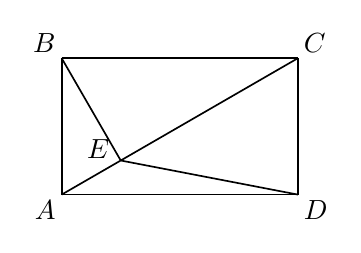
\begin{tikzpicture}[x=1cm,y=1cm,font=\normalsize,
 geometry edge/.style={solid,line width=.6pt},
 geometry mark/.style={solid,line width=.6pt},
 geometry label/.style={font=\normalsize,inner sep=2pt}]
\coordinate (A) at (0,0);
\coordinate (B) at (0,1.7321);
\coordinate (C) at (3,1.7321);
\coordinate (D) at (3,0);
\coordinate (E) at (0.75,0.433);
\draw[geometry edge] (A)--(B);
\draw[geometry edge] (B)--(C);
\draw[geometry edge] (C)--(D);
\draw[geometry edge] (D)--(A);
\draw[geometry edge] (A)--(E);
\draw[geometry edge] (E)--(C);
\draw[geometry edge] (B)--(E);
\draw[geometry edge] (E)--(D);
\node[geometry label,below left] at (A) {$A$};
\node[geometry label,above left] at (B) {$B$};
\node[geometry label,above right] at (C) {$C$};
\node[geometry label,below right] at (D) {$D$};
\node[geometry label,left,xshift=-2pt,yshift=4pt] at (E) {$E$};
\end{tikzpicture}
